\chapter{分离与可数}

\section{正则空间和正规空间}
\begin{definition}[正则空间]
    一个拓扑空间 $X$ 称为\textbf{正则的}, 如果
    \begin{enumerate}
        \item[(i)] $X$ 中的单点集是闭集;
        \item[(ii)] 对任意 $a \in X$ 和 $X$ 中的任意闭集 $B$ 且 $a \notin B$, 存在不相交的开集 $U$ 和 $V$ 使得 $a \in U$ 且 $B \subset V$.
    \end{enumerate}
\end{definition}
\begin{figure}[h]
    \centering
    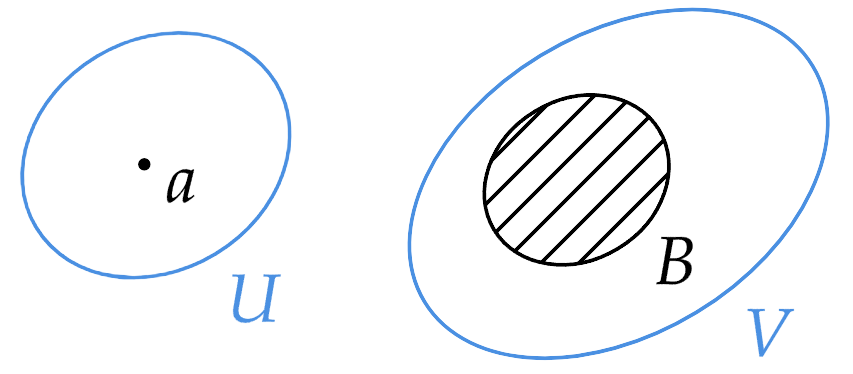
\includegraphics[width=0.35\textwidth]{fig/5.1.png}
    \caption{正则空间}
\end{figure}

\begin{remark}
    正则 $\implies$ Hausdorff.
\end{remark}

\begin{definition}[正规空间]
    一个拓扑空间 $X$ 称为\textbf{正规的}, 如果
    \begin{enumerate}
        \item[(i)] $X$ 中的单点集是闭集;
        \item[(ii)] 对任意两个不相交的闭集 $A, B \subset X$, 存在不相交的开集 $U$ 和 $V$ 使得 $A \subset U$ 且 $B \subset V$.
    \end{enumerate}
\end{definition}
\begin{figure}[h]
    \centering
    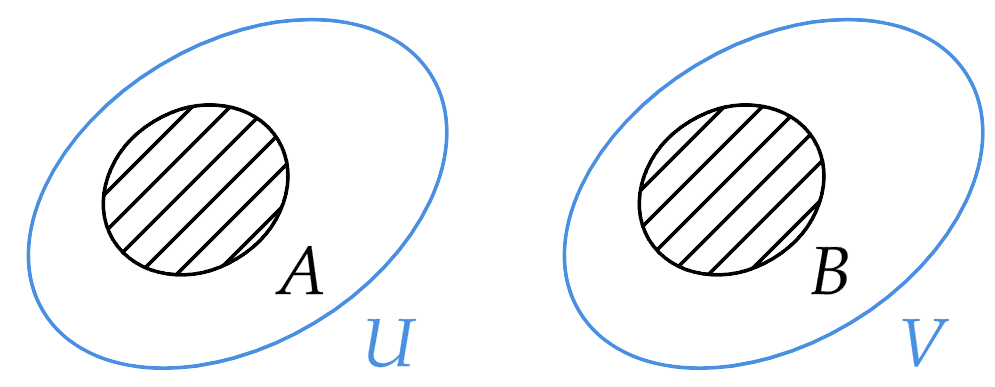
\includegraphics[width=0.35\textwidth]{fig/5.2.png}
    \caption{正规空间}
\end{figure}

\begin{remark}
    正规 $\implies$ 正则.
\end{remark}

\section{分离公理}

我们也称 Hausdorff 空间为 $T_2$ 空间, 正则空间为 $T_3$ 空间, 正规空间为 $T_4$ 空间，它们都反应了拓扑空间的分离性质，并且有以下包含关系:
\begin{axiom}{分离公理}
    正规 ($T_4$) $\subset$ 正则 ($T_3$) $\subset$ Hausdorff ($T_2$)
\end{axiom}

上一节章中证明了每个度量空间都是 Hausdorff 的，现在可以进一步证明每个度量空间都是正规的，也就是度量空间有最强的分离性质.\par
\begin{proposition}
    任意一个度量空间都是正规的.
\end{proposition}
\begin{proof}
    首先，对$\forall\, x\in X,y\in X-\{x\}$，$d(x,y)>0$，则$y\in B\left(y,d(x,y)\right)\subset X-\{x\}$，因此$X-\{x\}$是一个开集，从而单点集$\{x\}$是闭集.\par
    假设 $X$ 是一个度量空间, $A$ 和 $B$ 是 $X$ 中两个不相交的闭集.定义如下函数：
    {\setjot[-7]\begin{align*}
        g: X &\to \mathbb{E}^1 \\ 
        x &\mapsto d(x, A) := \inf\{d(x, a) \mid a \in A\} \\
        h: X &\to \mathbb{E}^1 \\ 
        x &\mapsto d(x, B) := \inf\{d(x, b) \mid b \in B\} \\
        f: X &\to \mathbb{E}^1 \\
        x &\mapsto \frac{d(x, A)}{d(x, A) + d(x, B)}
    \end{align*}}\par
    \hspace{-1.5em}(i)\; 证明 $g$ 和 $h$ 是连续的.即对$\forall\,(r, s) \subset \mathbb{E}^1$, $g^{-1}((r, s))$ 在 $X$ 中是开集.\par
    也就是$\forall\,x \in g^{-1}((r, s))$，我们需要证明$\exists\,\varepsilon > 0$ 使得 $x \in B(x, \varepsilon) \subset g^{-1}((r, s))$.
    \begin{center}
        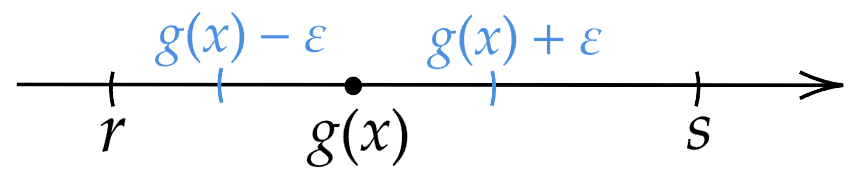
\includegraphics[width=0.35\textwidth]{fig/5.3.png}
        \captionof{figure}{}
    \end{center}\par
    由$g(x) \in (r, s)$，可取$\varepsilon > 0$ 使得$(g(x)-\varepsilon, g(x)+\varepsilon) \subset (r, s)$，即 $g(x)-\varepsilon > r$ 且 $g(x)+\varepsilon < s$.\par        
    那么$\forall\,y \in B(x, \varepsilon)$，有$d(x, y) < \varepsilon$，则$\setjot[-4]\begin{aligned}[t]
        g(y) &= d(y, A) = \inf\{d(y, a) \mid a \in A\}  \\
        &\leq \inf\{d(y, x) + d(x, a) \mid a \in A\} \\
        &= d(y, x) + d(x, A) < \varepsilon + g(x) < s
        \end{aligned}$.\par
    另一方面，$g(x) = d(x, A) \leq d(x, y) + d(y, A) < \varepsilon + g(y) \implies g(y) > g(x) - \varepsilon > r$.\par
    因此 $g(y) \in (r, s)$, 所以 $B(x, \varepsilon) \subset g^{-1}((r, s))$.
    这证明了 $g^{-1}((r, s))$ 是开集, 所以 $g$ 是连续的.\par
    同理, $h$ 也是连续的.\par
    \hspace{-1.8em}(ii)\; 证明$\forall\,x \in X$, $d(x, A) + d(x, B) > 0$.
    等价于证明 $d(x, A) + d(x, B) \neq 0$.\par
    \begin{minipage}[t]{0.765\textwidth}
         先证$d(x, A) = 0 \iff x \in A$.\par
    “$\Leftarrow$”显然.\par
    “$\Rightarrow$”设$x\notin A$.由于$A$是闭集，$X-A$是开集，故$\exists\, \delta>0,\st B(x,\delta)\subset X-A$.\par
    则$d(x,A)\geq \delta>0$，矛盾!\par
    \end{minipage}
    \begin{minipage}[t]{0.18\textwidth}
        \vspace{-3em}
        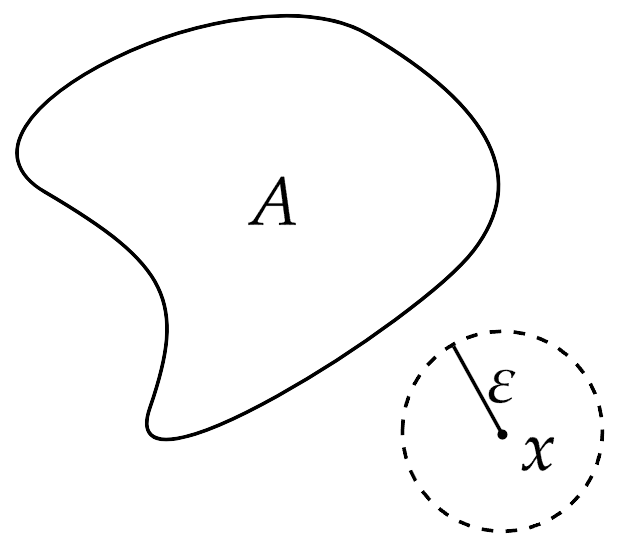
\includegraphics[width=1\textwidth]{fig/5.4.png}
        \captionof{figure}{}
    \end{minipage}\par
    如果 $d(x, A) + d(x, B) = 0$, 那么必有 $d(x, A) = 0$ 和 $d(x, B) = 0$. \par
    这意味着 $x \in A$ 且 $x \in B$, 即 $x \in A \cap B$.但这与 $A \cap B = \emptyset$ 矛盾.\par
    (ii)证明了$f$的分母恒不为零.\par    
    由 (i) 和 (ii), 函数 $f$ 是连续的 (因为它是连续函数的和、商, 且分母不为零).\par
    对$\forall\,a \in A$，$d(a,A)=0$，故$f(a) = \frac{d(a, A)}{d(a, A) + d(a, B)} = \frac{0}{0 + d(a, B)} = 0$.\par
    对任意 $b \in B$，$d(b,B)=0$，故$f(b) = \frac{d(b, A)}{d(b, A) + d(b, B)} = \frac{d(b, A)}{d(b, A) + 0} = 1$.\par
    令 $U = f^{-1}\left(\left(-\infty, \frac{1}{2}\right)\right)$ 和 $V = f^{-1}\left(\left(\frac{1}{2},+\infty\right)\right)$.
    因为 $f$ 是连续的, $U$ 和 $V$ 都是开集.
    并且 $A \subset U$, $B \subset V$, 且 $U \cap V = \emptyset$.
    这就证明了 $X$ 是正规空间.
\end{proof}

\section{可数性}
\begin{definition}[可数邻域基]
    拓扑空间 $X$ 在点 $x \in X$ 处有\textbf{可数邻域基}, 如果存在 $x$ 的一个可数邻域族 $\{U_n\}_{n \in \mathbb{Z}^+}$ 使得 $x$ 的任何邻域 $W$ 都包含其中一个 $U_n$, 即 $x \in U_n \subset W$.
\end{definition}

\begin{definition}[第一可数]
    如果 $X$ 在其每一点都有可数邻域基, 则称 $X$ 是\textbf{第一可数的}, 或满足\textbf{第一可数性公理}.
\end{definition}

\begin{example}
    每个度量空间都是第一可数的.对任意 $x \in (X, d)$, $\{U_n = B(x, 1/n)\}_{n \in \mathbb{Z}^+}$ 是一个可数邻域基.
\end{example}

\begin{definition}[第二可数]
    如果一个空间 $X$ 的拓扑有一个可数的基, 那么 $X$ 称为\textbf{第二可数的}, 或满足\textbf{第二可数性公理}.
\end{definition}

\begin{example}
    $\mathbb{R}^n$ 是第二可数的.一个可数基是 $\mathcal{B} = \{B(x, 1/k) \mid x \in \mathbb{Q}^n, k \in \mathbb{Z}^+\}$.
\end{example}
